\insertdesignoverview{Hang Winch}
{Create a fast, reliable hang mechanism to latch and de-latch in both autonomous and endgame} % Goals of the mechanism
{Hang.PNG}% CAD Image
{fullbullseyehang.PNG}% Build Image
{Steel rods, Duracord, Surgical Tubing, Aluminum}% Materials ex. 0.25" MDF, Aluminum, etc
{Laser Cutting, CNC Milling, Metal Bending}% Manufacturing Processes ex. Laser Cut, 3D print, etc.

%\interesting{Our innovative glyph delivery mechanism, analyzed in depth}{Innovate:55}

\subsection*{How it Works}
The hang mechanism works by attaching a hook onto the end of the front arm. This hook has a winch connected to it that runs through the robot and to the underside where a 40:1 motor turns, lifting the robot. The claw gets to the latch by tilting the robot so that the front arm sticks up in the air. The claw than rotates due to a small servo on the arm to put the hook into the latch when the winch motor pulls the robot up. In autonomous, the winch motor spins the opposite way to lower the robot and unhooks by tilting the robot to push up. 

 \begin{figure}[h!]
 \centering
   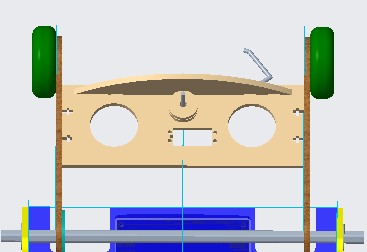
\includegraphics[width=0.8\textwidth, angle=0]{Design_Overview/Hang_1.PNG}
  \caption{Hang Top Pic}
  \label{fig:hang_top}
 \end{figure}

\subsection*{Modelling \& Simulation}
Modelling the hang mechanism involved minimal design challenges. The only thing we originally struggled with was how the arms would line up with the lander. In order to model this, we used body and motion skeletons to see the distance to the latch as well as how far in it would reach. However, issues were primarily resolved through design iteration, as you'll see below. 

\subsection*{Iteration}
Initially,we angled the hang plate that held the hook, believing that that would allow for the hook to be well within the latch. However, after testing, we determined that a straight hang plate worked much better. We also made several iterations of a winch box that would rest at the back of the chassis, yet after struggling with space issues we realized that we could simply mount the motor directly on the underbelly of the chassis with a hole to guide the winch string.

\begin{figure}[htp]
\centering
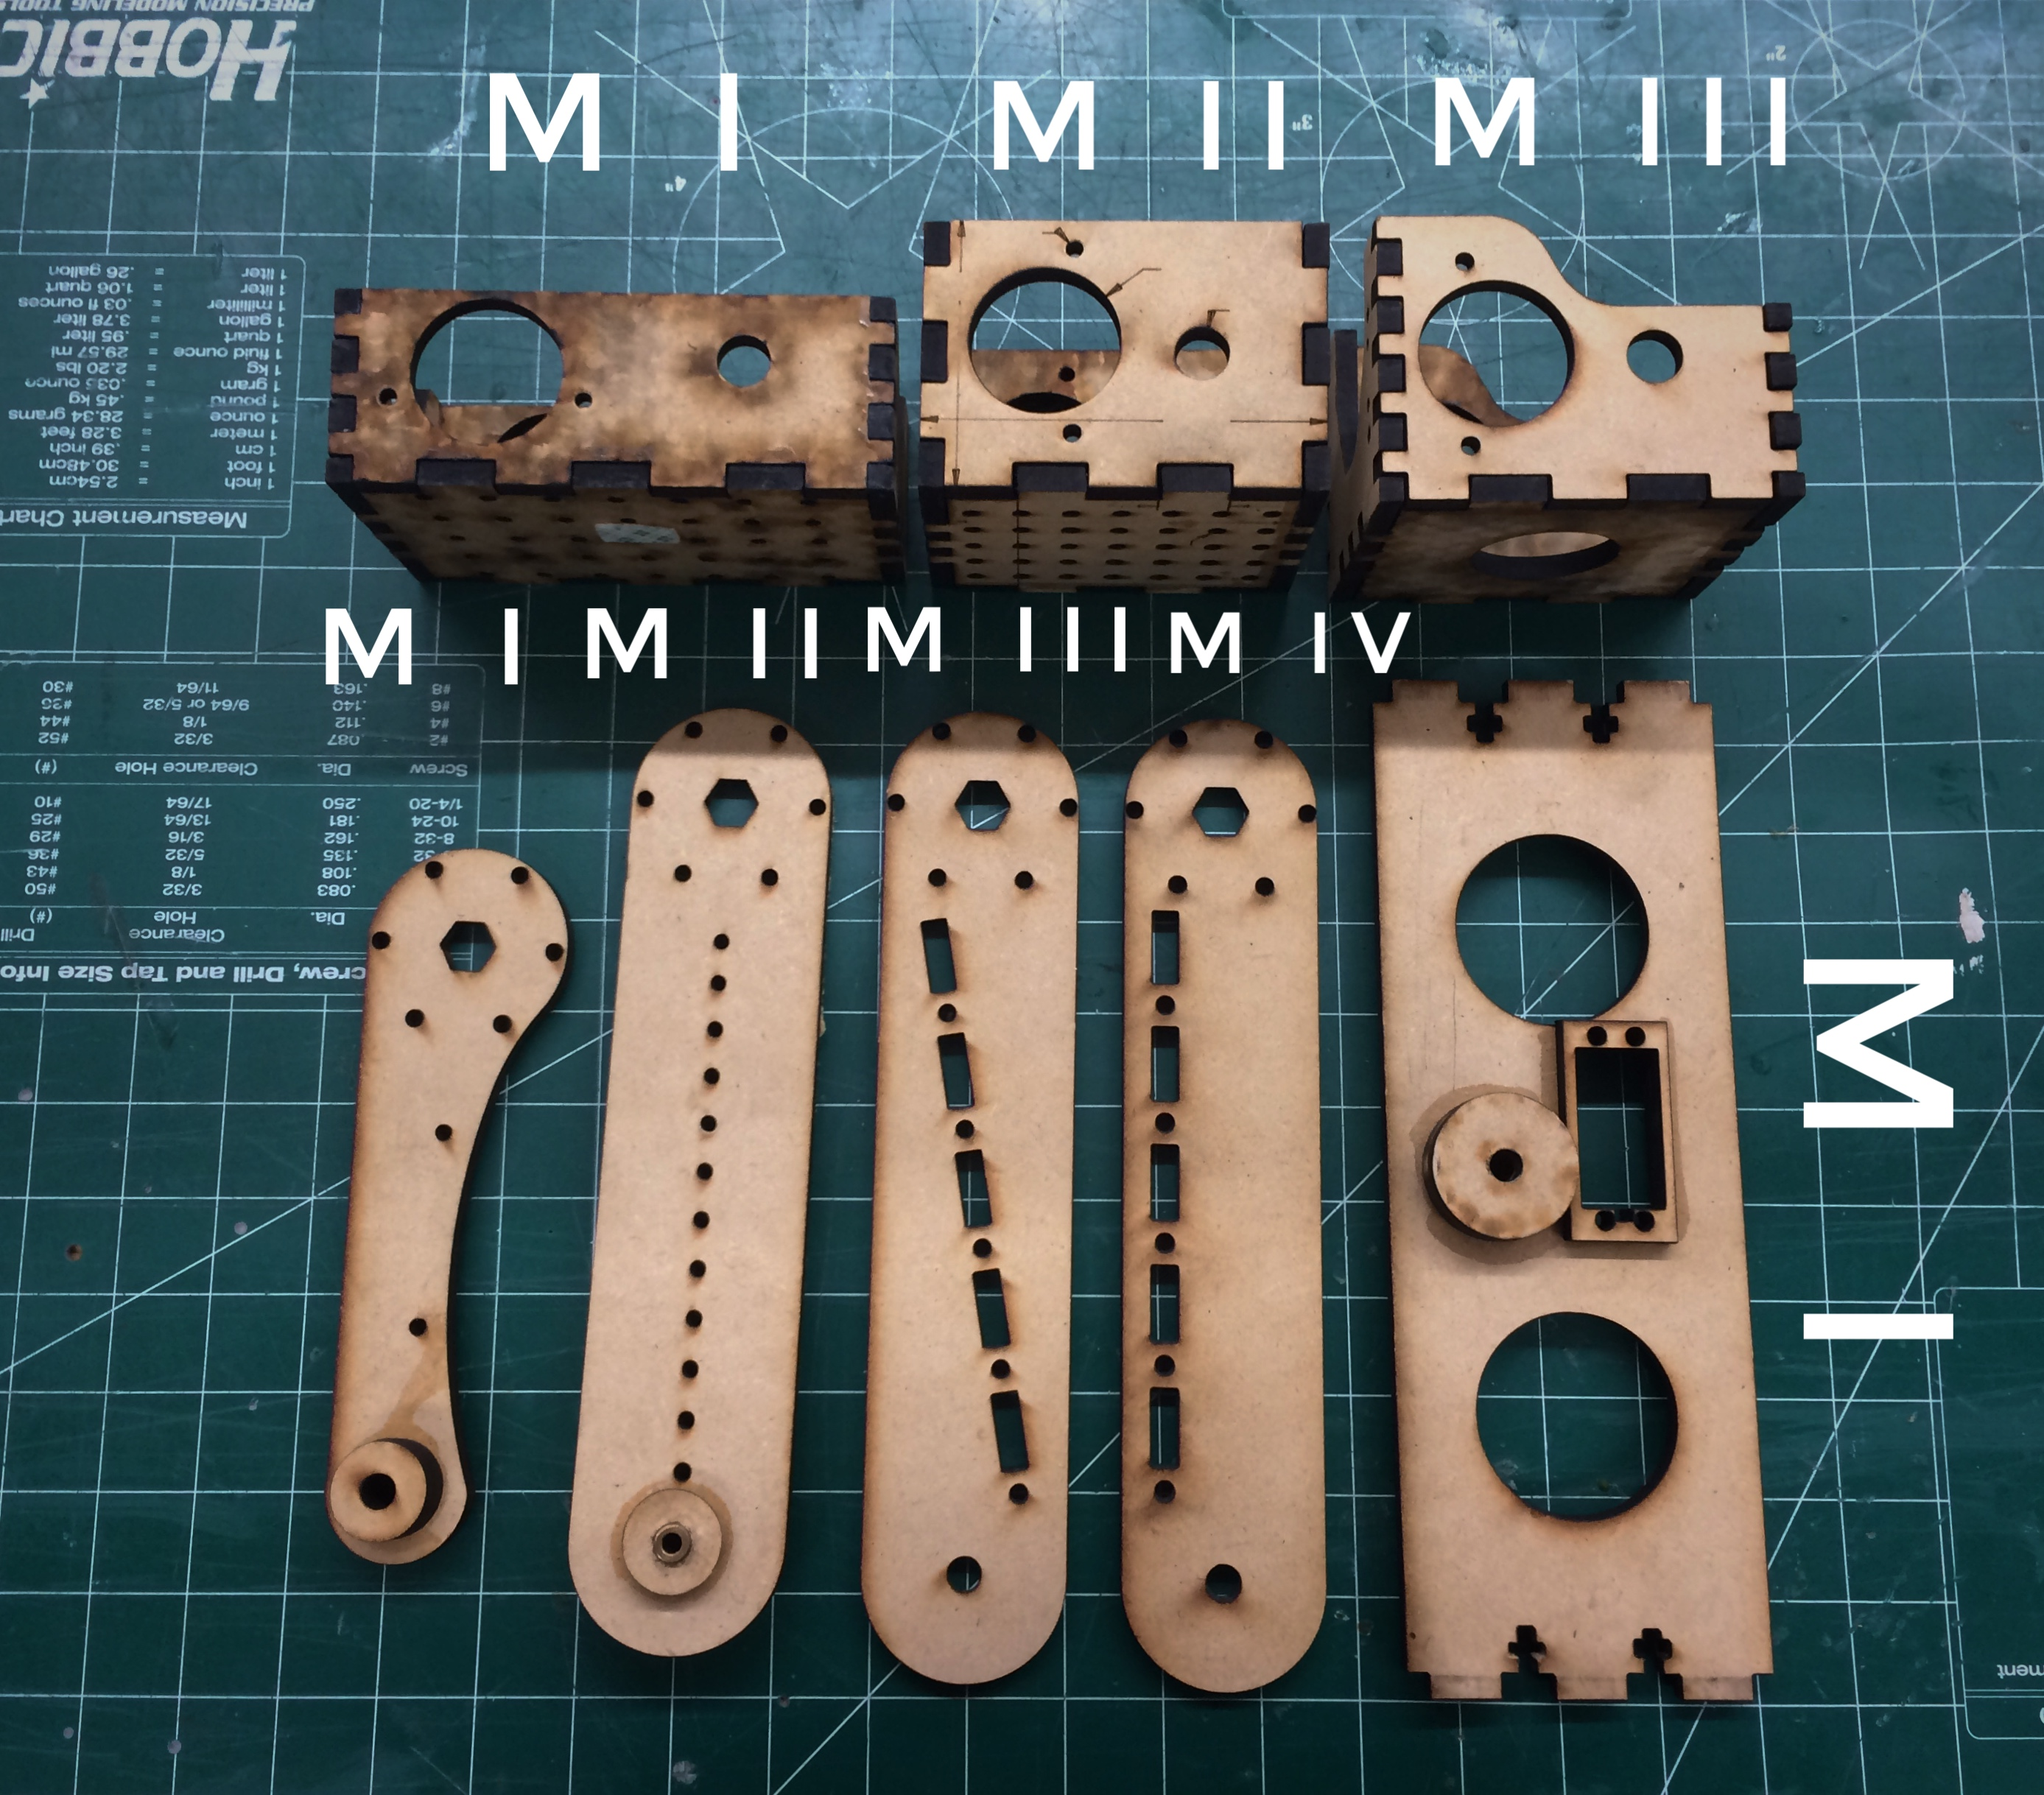
\includegraphics[width=.8\linewidth]{Design_Overview/Hang_Iteration.jpg}
\caption{Design Iteration of the Hang, Mark I to Mark IV}
\label{fig:hang_iteration}
\end{figure}

\begin{figure}[htp]
\centering
\begin{minipage}{.32\textwidth}
  \centering
  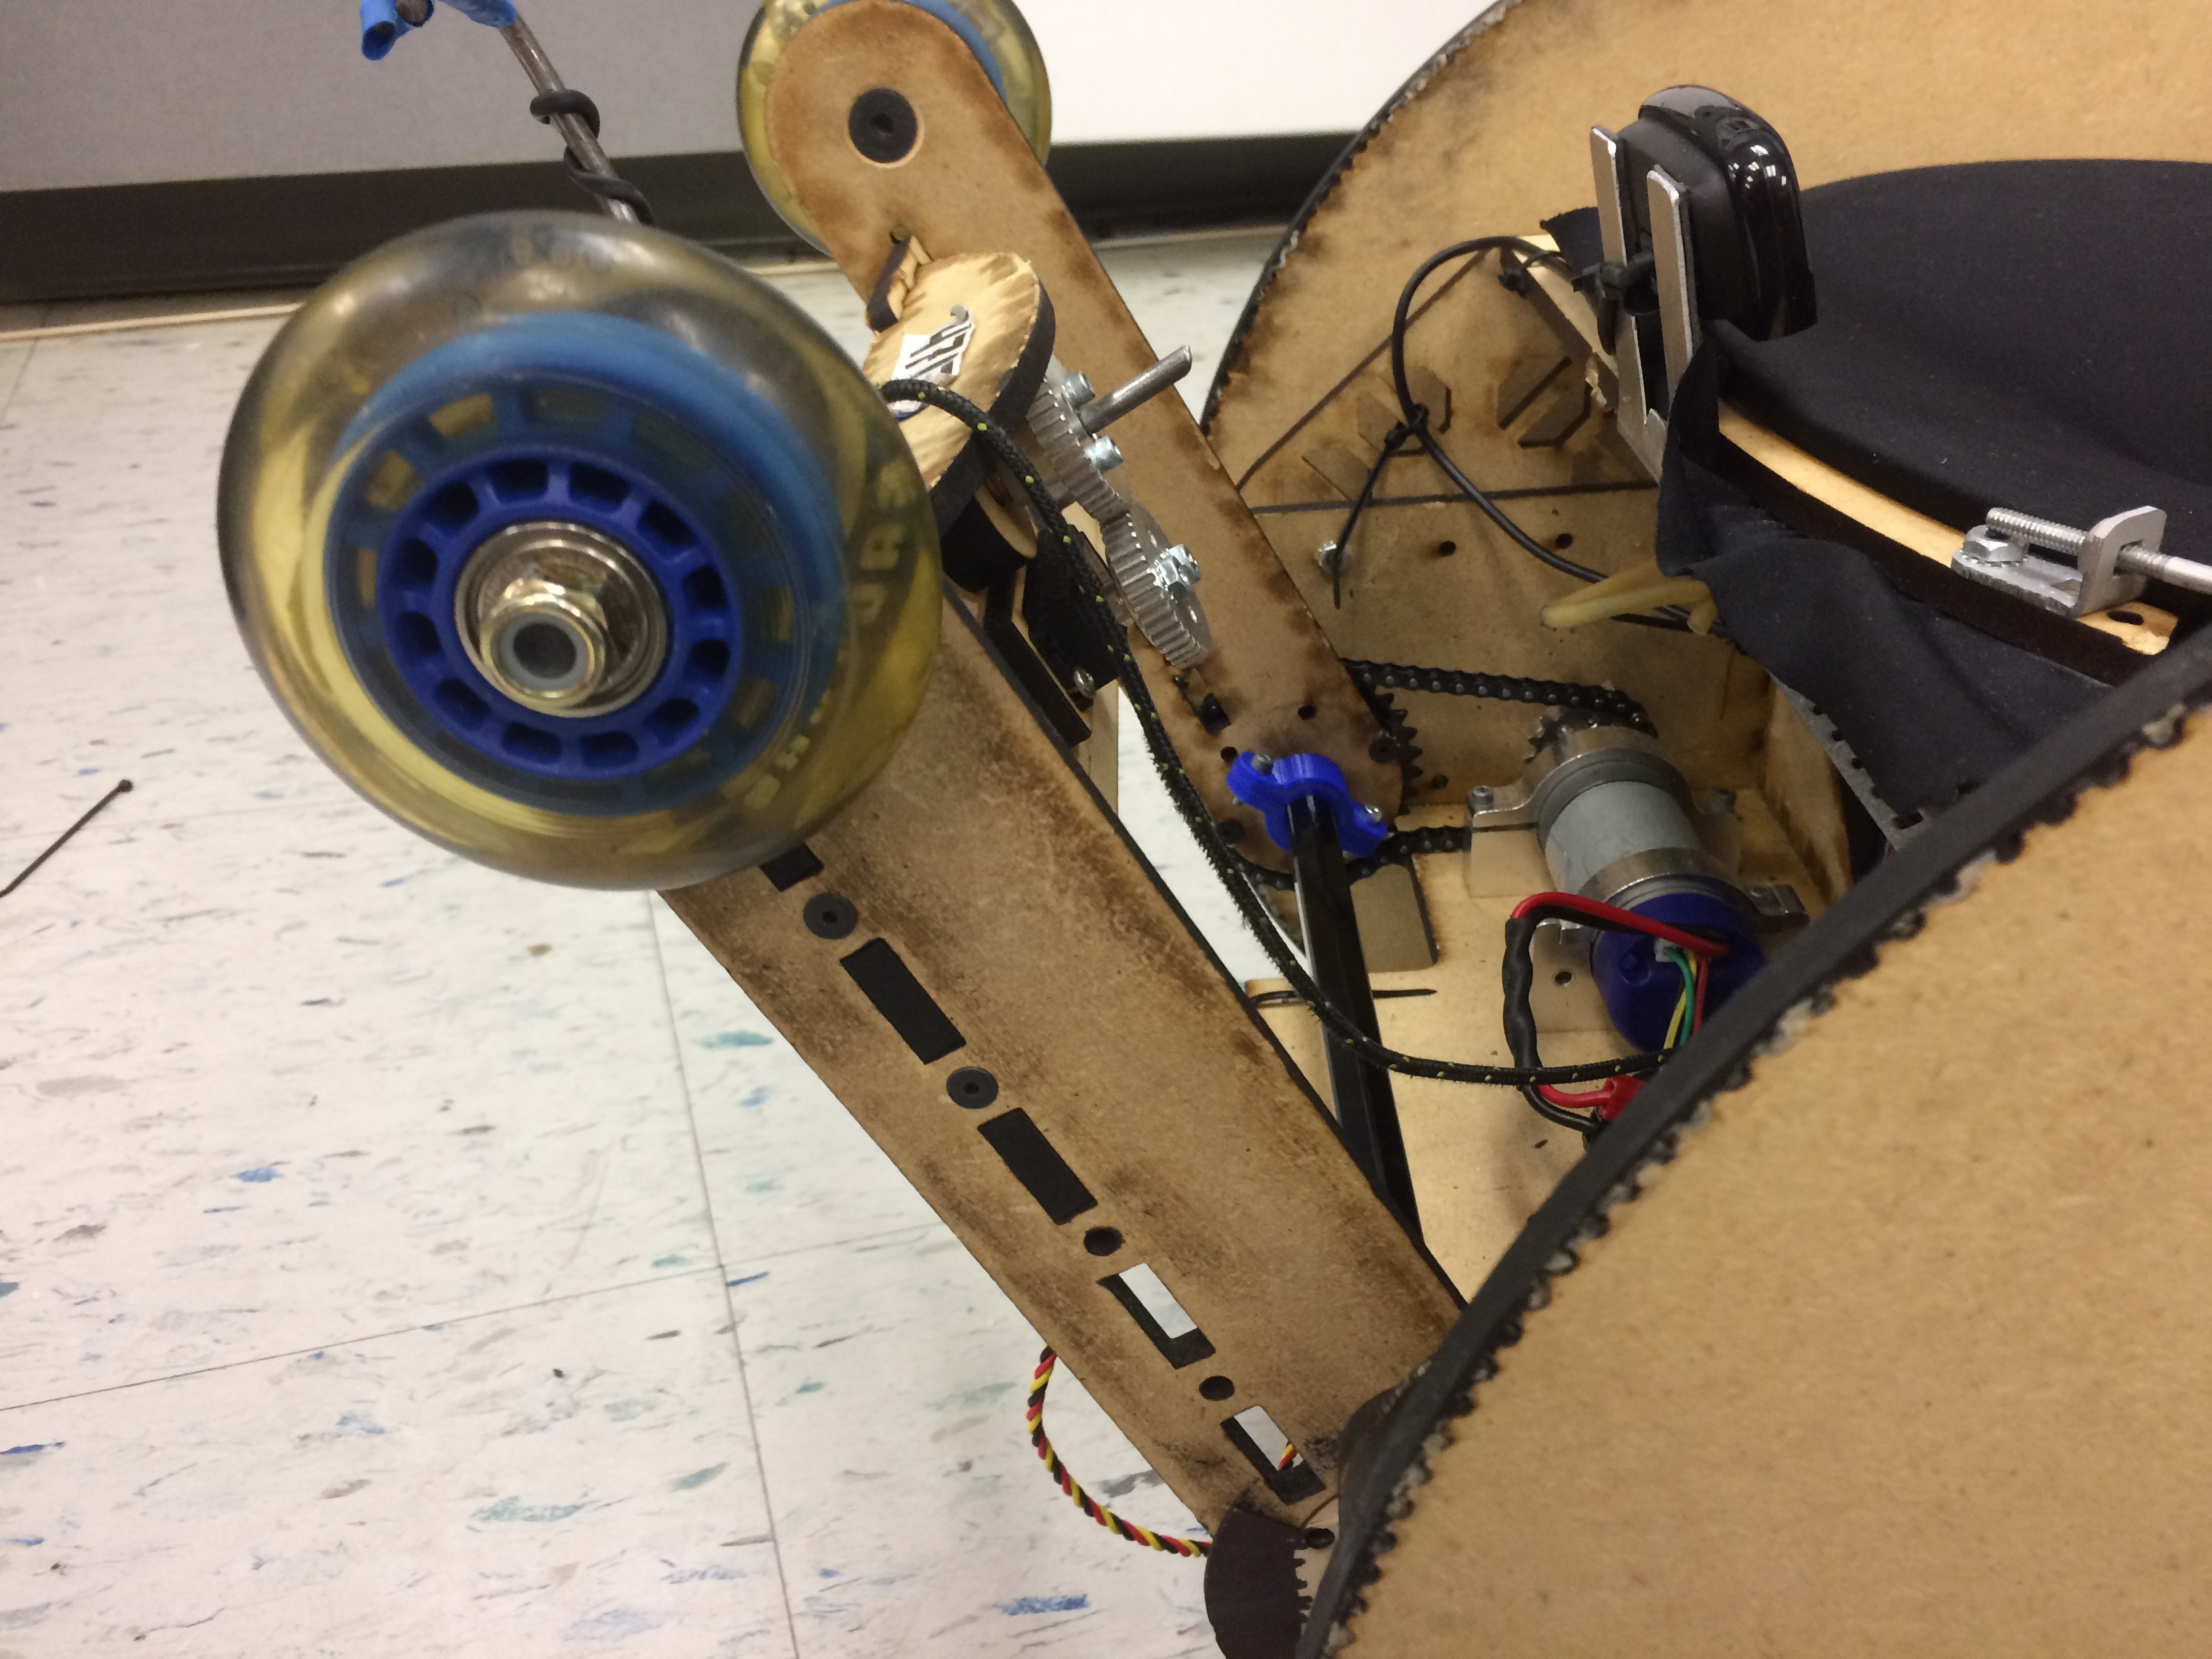
\includegraphics[width= .9\linewidth]{Design_Overview/Hang_Left.JPG}
\end{minipage}%
\hfill
\begin{minipage}{.32\textwidth}
  \centering
  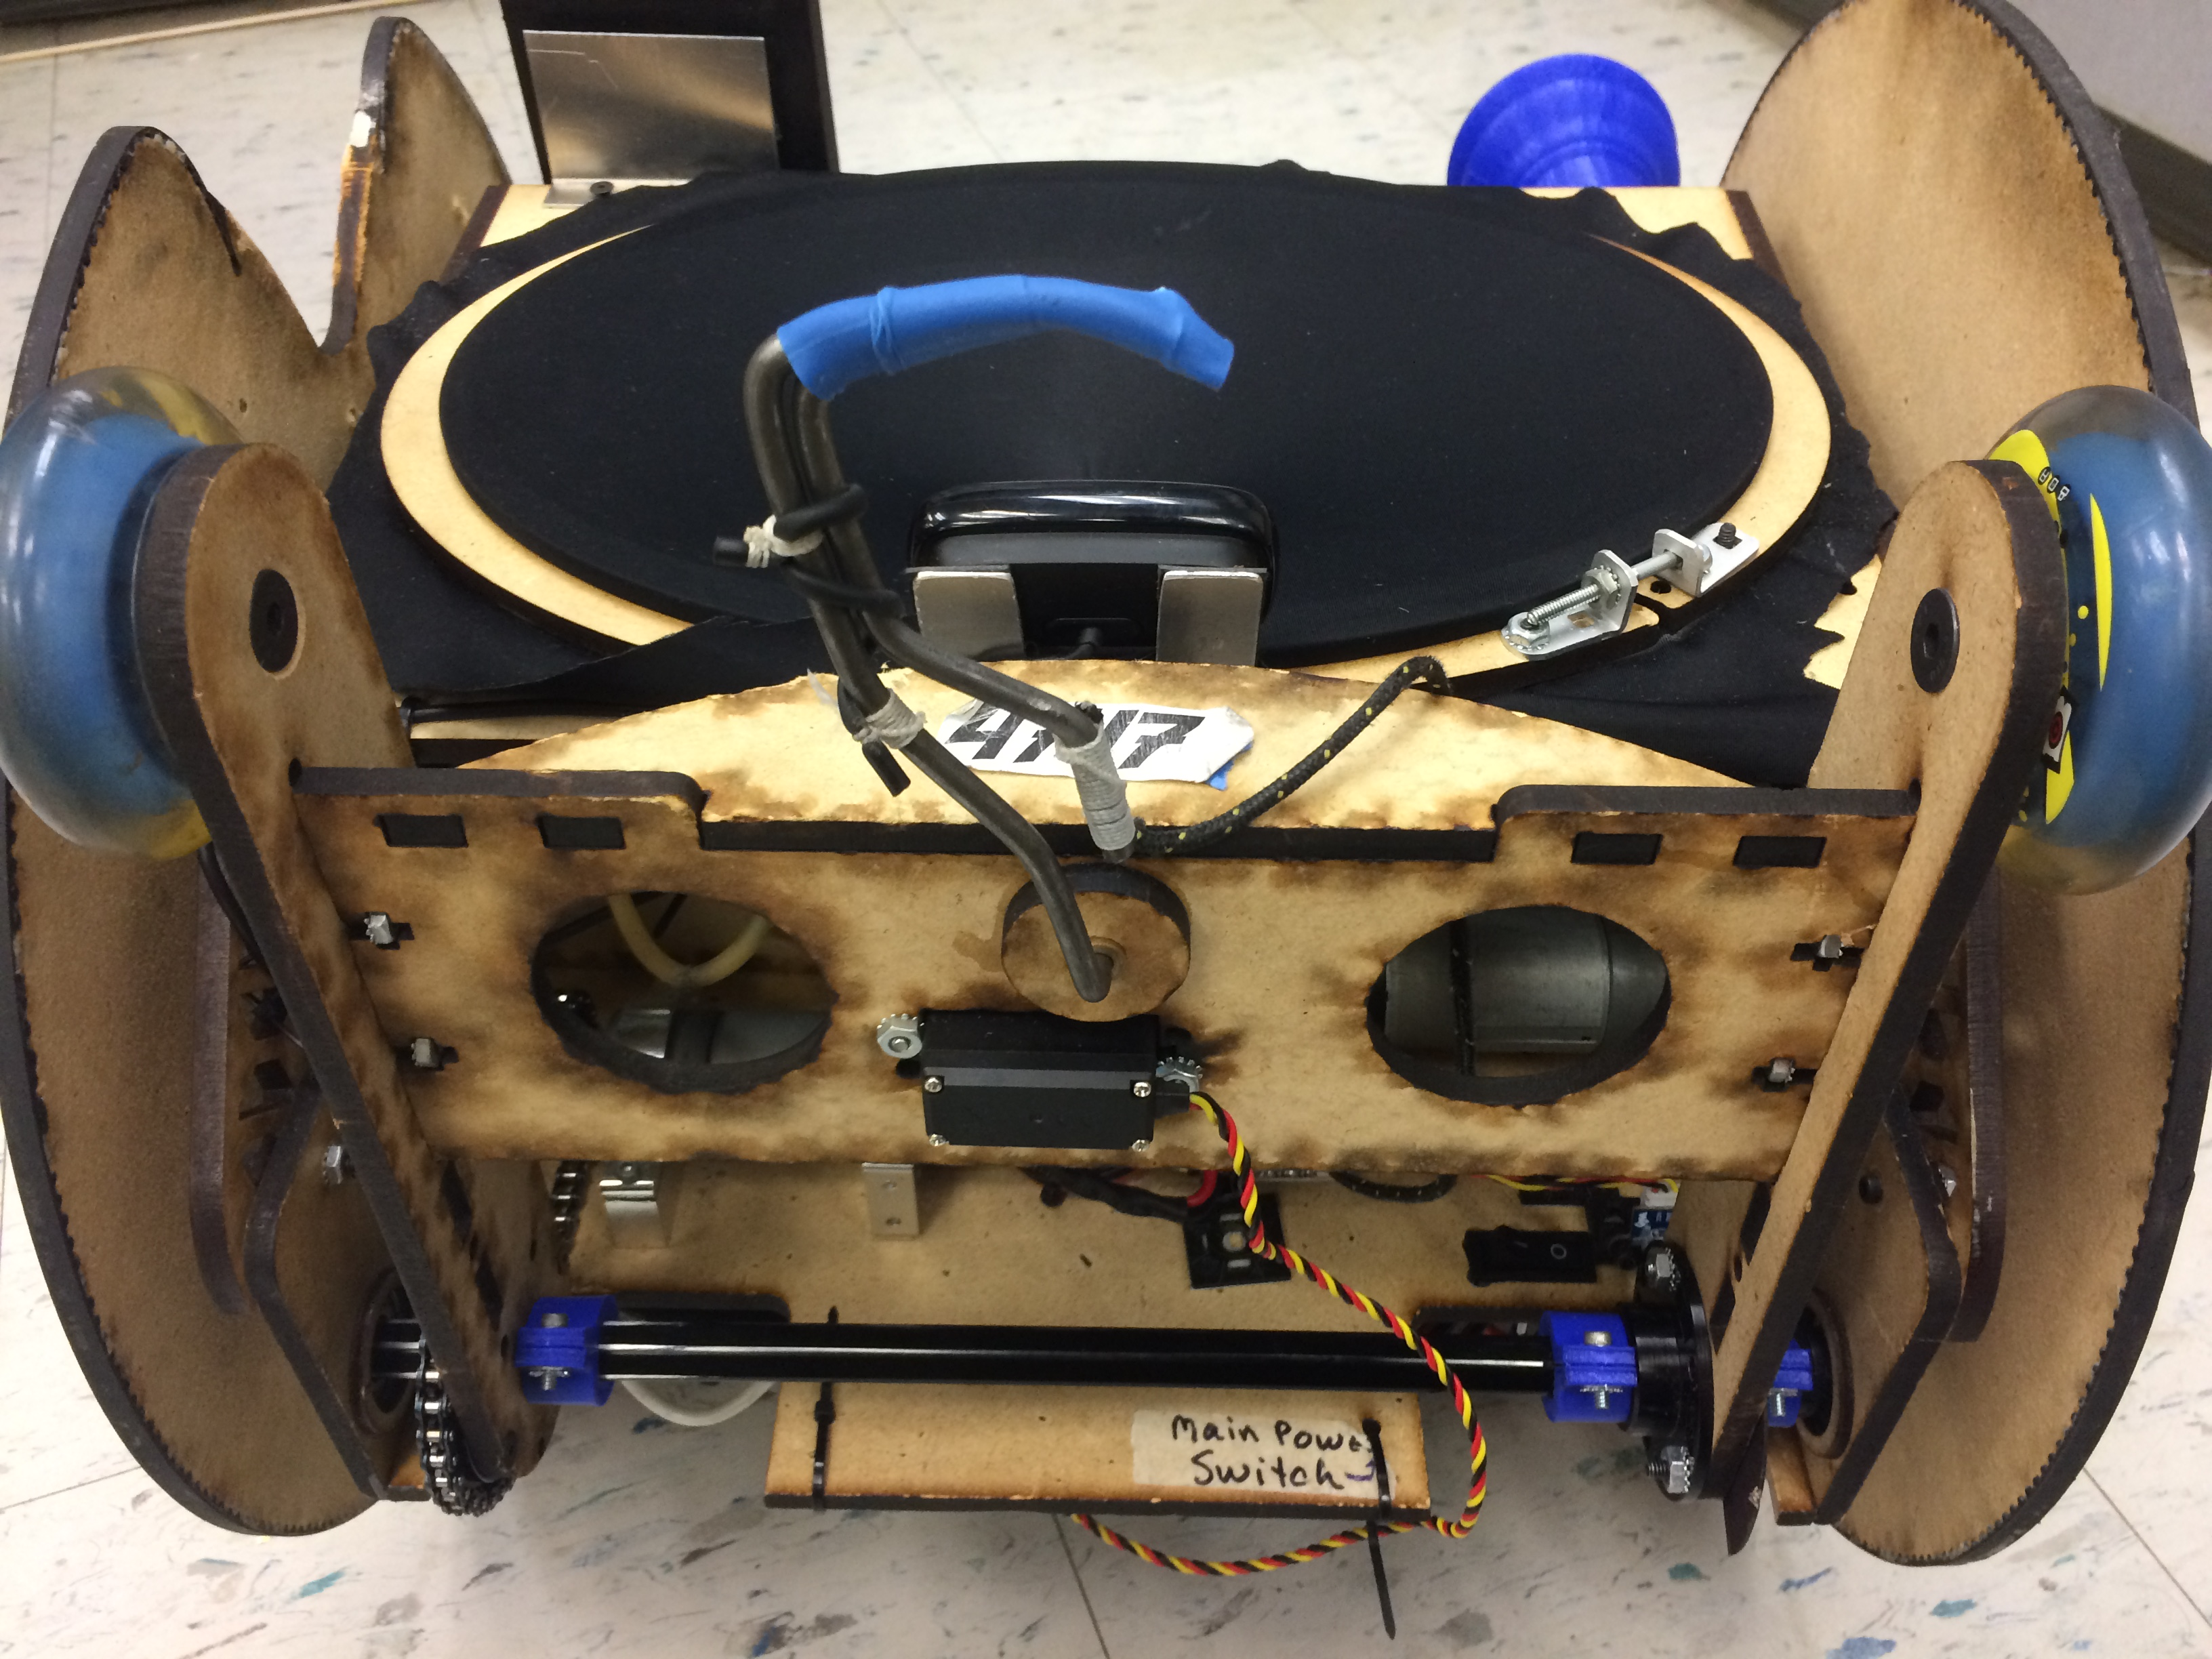
\includegraphics[width= .9\linewidth]{Design_Overview/Hang_Front.JPG}
	\caption{Final Hang Mechanism, Mark V}
	\label{fig:hang_final_IMG}
\end{minipage}%
	\hfill
\begin{minipage}{.32\textwidth}
  \centering
  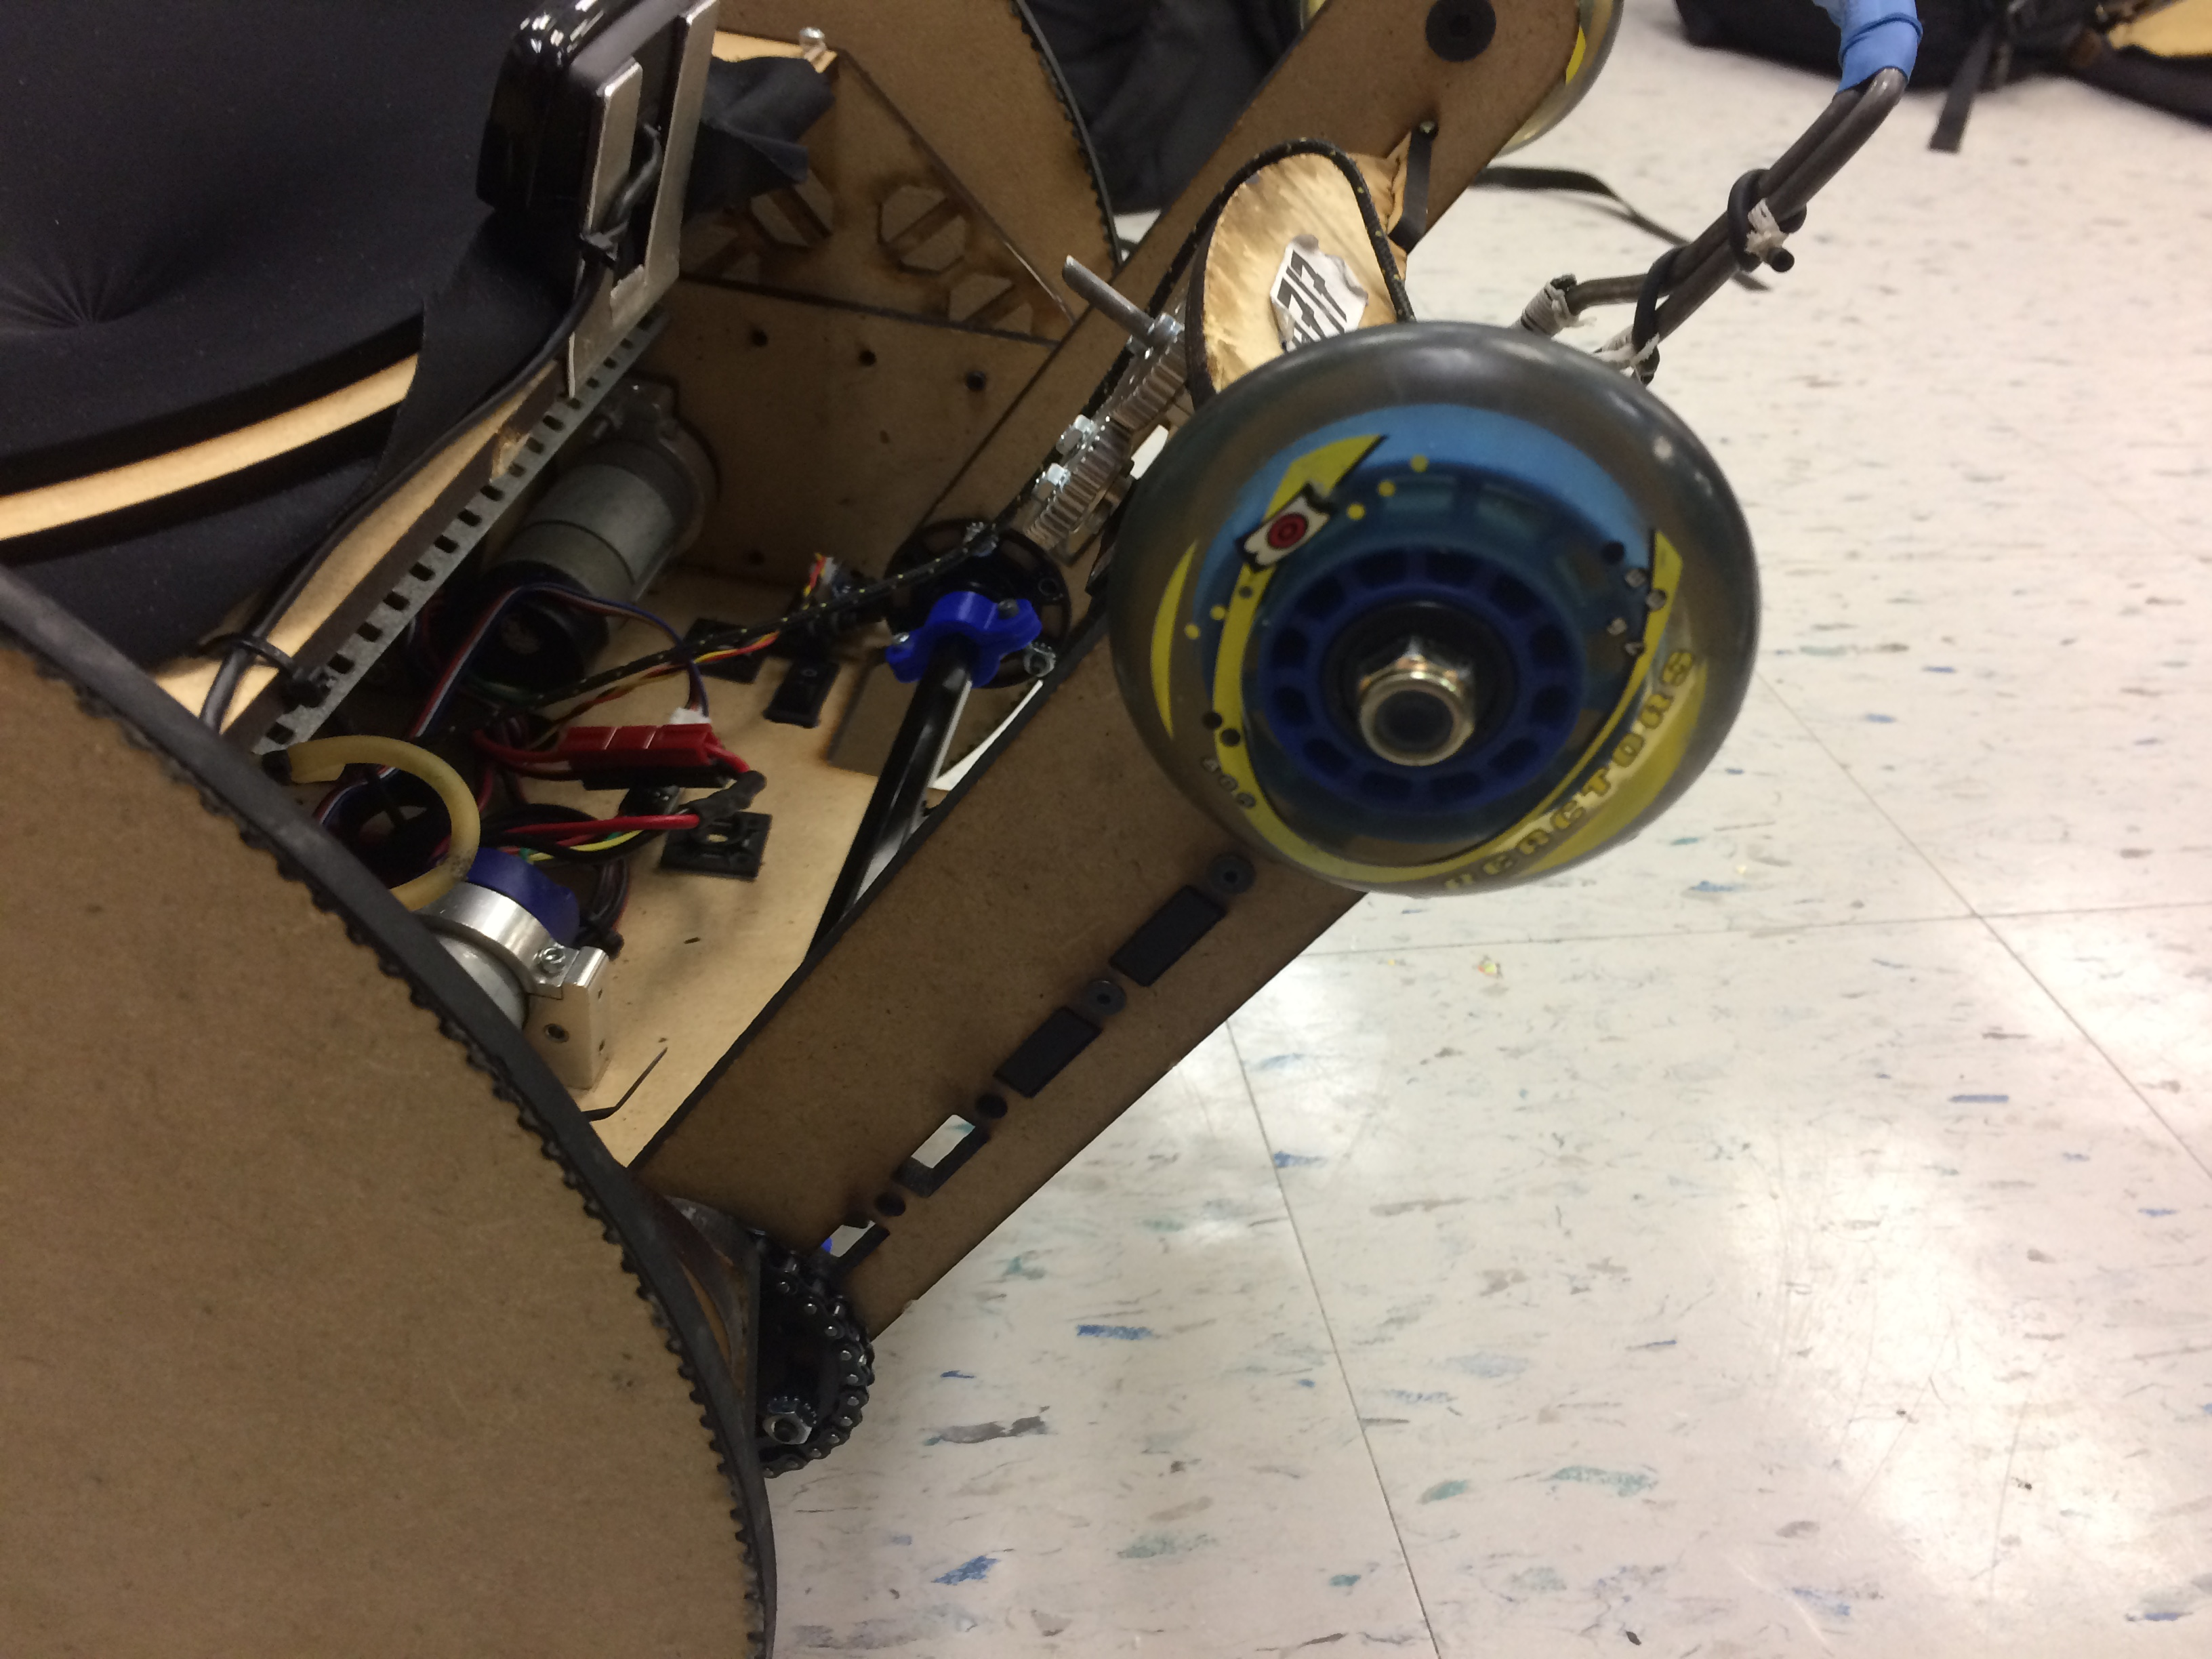
\includegraphics[width= .9\linewidth]{Design_Overview/Hang_Right.JPG}
\end{minipage}
\end{figure}

\subsection*{Sensors and Control}
The winch motor uses encoder PID to hold the hang position during autonomous. In addition, we use two buttons for autonomous setup, with the buttons controlling winching up or winching down. Wanting to determine the power of the motor, our physics team developed a formula to determine the amount of torque that the motor needs to pull the horn down. These equations are described below. 
